\chapter{Introducción}
%%---------------------------------------------------------

\section{Contexto y motivación del proyecto}


En esta primera parte del proyecto se intentarán poner en perspectiva, de una forma no exhaustiva, las distintas razones
históricas que dan lugar a la necesidad de crear un sistema de almacenamiento descentralizado y distribuido como IPFS.
Para ello, se hará un breve repaso histórico de la evolución de Internet y de los protocolos que lo han ido conformando.
Posteriormente, se explicará la tendencia centrlista del sistema actual, existente a un nivel íntrinseco y estructural,
además de otros problemas que se derivan de esta situación.
Finalmente, se expondrá la propuesta de solución que IPFS ofrece para solventar estos problemas, sobre la que se profundizará en el capítulo \ref{chap:ipfs} dedicada a IPFS .

\subsection{Predominancia de los protocolos TCP/IP}
La historia de Internet está marcada por la competencia entre distintos protocolos de comunicación que buscaban establecerse
como el estándar para intercambiar información entre diferentes redes y sistemas. Uno de los episodios más relevantes de esta
competencia fue la llamada \textit{"Guerra de los protocolos"} \cite{ProtocolWars2023}, en la que el conjunto de protocolos TCP/IP, creado entre los
años 1973 y 1974 por Vint Cerf y Robert Kah, se enfrentó a otras propuestas como OSI, X.25 o SNA\footnote{En la figura \ref{tab:comparacion-protocolos-90} de la página \pageref{tab:comparacion-protocolos-90} se muestra un resumen de las principales características de cada uno de estos protocolos.
}.

TCP/IP logró imponerse en la competencia debido a las siguientes características principalmente:
\begin{itemize}
      \item \textbf{ Interoperabilidad }: La capacidad de TCP/IP para conectarse fácilmente con diferentes tipos de ordenadores y sistemas operativos le otorgaba una ventaja sobre otros protocolos que eran más específicos o limitados en su compatibilidad. Esta característica permitía que diversas tecnologías y plataformas pudieran comunicarse entre sí sin problemas, lo cual era esencial para crear una red global como Internet.

      \item \textbf{ Flexibilidad }: TCP/IP podía adaptarse a distintos medios de transmisión, como cables de cobre, fibra óptica o incluso enlaces inalámbricos, lo que facilitaba su implementación en una amplia variedad de entornos y situaciones. Otros protocolos, en cambio, podrían haber requerido modificaciones o adaptaciones específicas para funcionar en diferentes tipos de medios de transmisión.

      \item \textbf{ Resistencia }frente a fallos: TCP/IP fue diseñado para ser robusto en caso de fallos en la red, permitiendo que los paquetes de datos pudieran ser retransmitidos y encontrar rutas alternativas en caso de problemas. Esta capacidad de recuperación era fundamental para garantizar la continuidad y fiabilidad de las comunicaciones en una red global con múltiples nodos y enlaces.

      \item \textbf{ Escalabilidad }: TCP/IP podía soportar el crecimiento de la red al permitir la incorporación de nuevos nodos y enlaces sin afectar negativamente su rendimiento. Su diseño jerárquico y descentralizado facilitaba la expansión de la red y evitaba los cuellos de botella que podrían haberse producido con otros protocolos menos escalables.

\end{itemize}

Estas ventajas hicieron que TCP/IP se convirtiera en la opción preferida frente a otros protocolos, al ser una solución más versátil,
resistente y escalable para la creciente demanda de interconexión entre sistemas y redes en todo el mundo. Cabe destacar también que era una solución con arquitectura abierta, no propietaria y de uso gratuito, es decir, sin necesidad de pagar licencias por su uso \cite{edwardsFoundationInternetTCP2021}.

Como en toda guerra también hubo un trasfondo político. Este hecho suele ser ignorado al abordarse este tema desde un punto de vista puramente tecnológico.
Y es que en 1980, el Departamento de Defensa de Estados Unidos declaró TCP/IP como el estándar para todas las redes militares \cite{leinerBriefHistoryInternet1999}.
A esto se sumaron numerosas comunidades de investigación y universidades que adoptaron TCP/IP como su protocolo de comunicación, como por ejemplo, Stanford University, donde Vint Cerf colaboró con Robert Kahn en el diseño del protocolo \cite{leinerBriefHistoryInternet1999}; University of California, Los Angeles (UCLA), que participó en el desarrollo temprano y las pruebas de TCP/IP \cite{leinerBriefHistoryInternet1999}; y University College London (UCL), donde el profesor Peter Kirstein promovió el uso de TCP/IP en Europa y su equipo contribuyó al desarrollo y pruebas del protocolo \cite{moriPeterKirsteinObituary2020}.

Esta completa adopción del protocolo se dió por finalizada cuando ARPANET la precursora de la actual Internet y financiada por la Agencia de Proyec
tos de Investigación Avanzados de Defensa (DARPA), llevó a cabo la transición exitosa de su antiguo protocolo, el Network Control Program (NCP),
a TCP/IP el 1 de enero de 1983
\cite{leinerBriefHistoryInternet1999}.

En resumen, la rápida adopción de la comunidad científica y academéica, sumada al respaldo gubernamental consolidaron TCP/IP como el estándar dominante en la industria de las redes de comunicación.

\subsection{La World Wide Web y HTTP}
El modelo TCP/IP asentó una forma de comunicación estándar entre computadores y redes, aunque
este estaba limitado principalmente al mundo académico y científico. No fue hasta la creación de la World Wide Web (WWW)
cuando el Internet concebido como es en la actualidad se convirtió en un fenómeno global y accesible para todo el mundo.

Antes de la WWW, el acceso a la información en Internet se realizaba a través de los protocolos a nivel de aplicación mostrados en la figura \ref{fig:evolucion-protocolos}

\begin{table}[h!]
      \small
      \centering
      \begin{tabular}{>{\raggedright}m{3cm}m{10cm}}
            \toprule
            \textbf{Protocolo}                                   & \textbf{Descripción}                                                                                                                                                \\
            \midrule
            FTP (Protocolo de Transferencia de Archivos)         & Utilizado para transferir archivos entre cliente y servidor a través de una red.                                                                                    \\
            \addlinespace
            Telnet                                               & Basado en texto utilizado para el acceso remoto a computadoras y servidores, permitiendo a los usuarios controlarlos a través de una interfaz de línea de comandos. \\
            \addlinespace
            Gopher                                               & Diseñado para buscar y recuperar documentos de manera jerárquica, utilizando una interfaz basada en menús.                                                          \\
            \addlinespace
            SMTP (Protocolo Simple de Transferencia de Correo)   & Utilizado para enviar mensajes de correo electrónico entre servidores y, finalmente, al cliente de correo del destinatario.                                         \\
            \addlinespace
            NNTP (Protocolo de Transferencia de Noticias en Red) & Utilizado para la distribución, consulta y recuperación de artículos de noticias en la red Usenet.                                                                  \\
            \addlinespace
            POP3 (Protocolo de Oficina de Correos 3)             & Utilizado para recuperar mensajes de correo electrónico desde un servidor de correo remoto hasta un cliente de correo local.                                        \\
            \addlinespace
            IMAP (Protocolo de Acceso a Mensajes de Internet)    & Que permite a los usuarios acceder y administrar sus mensajes de correo electrónico en un servidor de correo, sin descargarlos a un cliente de correo local.        \\
            \bottomrule
      \end{tabular}
      \caption{Protocolos de capa de aplicación antes de HTTP}
      \label{fig:evolucion-protocolos}
\end{table}

. Estando estos servicios en el nivel de aplicación dentro del modelo TCP/IP \ref{fig}que ofrecían métodos básicos de navegación y compartición de archivos, pero carecían de la capacidad de interconectar
documentos de manera intuitiva y visual.

\usetikzlibrary{shapes,arrows,positioning, babel}



\begin{figure}[h!]
      \centering
      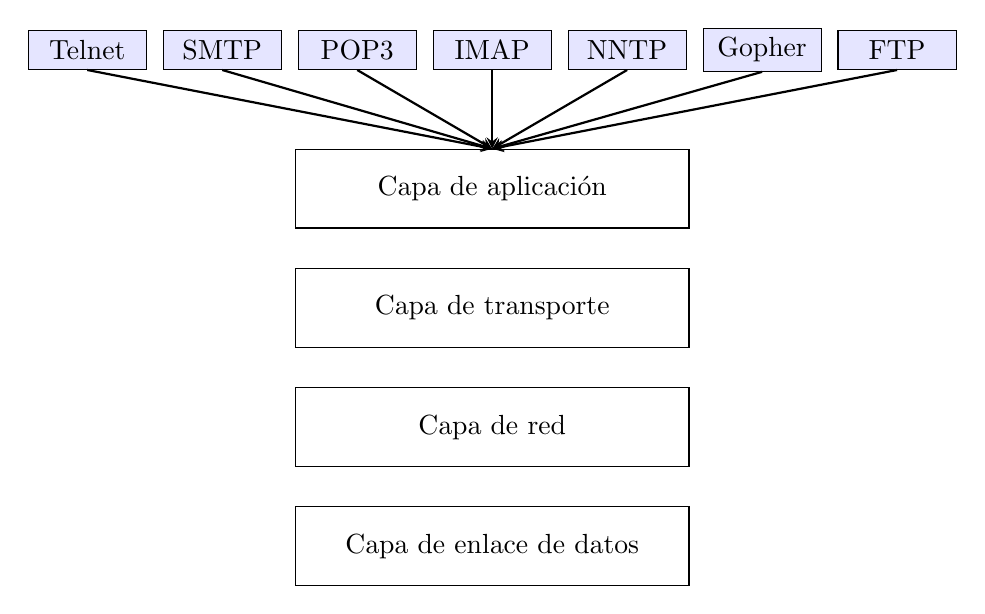
\begin{tikzpicture}
            % Estilos
            \tikzstyle{layer}=[draw, rectangle, minimum height=1cm, minimum width=5cm, text centered]
            \tikzstyle{app_protocol}=[draw, rectangle, minimum height=0.5cm, minimum width=1.5cm, text centered, fill=blue!10]
            \tikzstyle{arrow}=[->,>=stealth, thick]

            % Nodos
            \node[layer] (application) {Capa de aplicación};
            \node[layer, below=0.5cm of application] (transport) {Capa de transporte};
            \node[layer, below=0.5cm of transport] (network) {Capa de red};
            \node[layer, below=0.5cm of network] (link) {Capa de enlace de datos};

            \node[app_protocol, above=1cm of application.north] (imap) {IMAP};
            \node[app_protocol, left=0.2cm of imap] (pop3) {POP3};
            \node[app_protocol, right=0.2cm of imap] (nntp) {NNTP};
            \node[app_protocol, left=0.2cm of pop3] (smtp) {SMTP};
            \node[app_protocol, right=0.2cm of nntp] (gopher) {Gopher};
            \node[app_protocol, left=0.2cm of smtp] (telnet) {Telnet};
            \node[app_protocol, right=0.2cm of gopher] (ftp) {FTP};

            % Flechas
            \draw[arrow] (imap.south) -- (application.north);
            \draw[arrow] (pop3.south) -- (application.north);
            \draw[arrow] (nntp.south) -- (application.north);
            \draw[arrow] (smtp.south) -- (application.north);
            \draw[arrow] (gopher.south) -- (application.north);
            \draw[arrow] (telnet.south) -- (application.north);
            \draw[arrow] (ftp.south) -- (application.north);
      \end{tikzpicture}
      \caption{Capas del protocolo TCP/IP con protocolos de la capa de aplicación}
      \label{fig:tcpip}
\end{figure}


En 1989, el científico británico Tim Berners-Lee propuso la creación de la WWW, un sistema de información global e hipertextual
que permitiría a los usuarios navegar y acceder a documentos interconectados mediante enlaces.


\begin{figure}
      \centering
      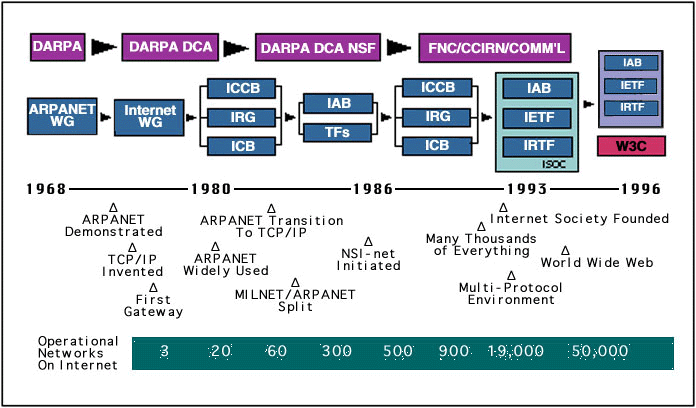
\includegraphics[width=0.8\textwidth]{images/TimelineOfTheInternetProtocols.png}
      \caption[Evolución de los protocolos de Internet]{Evolución de los protocolos de Internet. Fuente \cite{leinerBriefHistoryInternet1999}}
      \label{fig:evolucion-protocolos}
\end{figure}

Como se puede observar en la figura \ref{fig:evolucion-protocolos}

No obstante, el éxito de HTTP y la arquitectura centralizada de la web han generado ciertos desafíos y preocupaciones en cuanto a su eficiencia, fiabilidad y sostenibilidad. A medida que Internet se expande y se vuelve más complejo, la dependencia de servidores centralizados y la naturaleza volátil de la información en la web han llevado a la aparición de problemas como la lentitud en la distribución de contenidos, la fragilidad de los enlaces y nodos, y la tendencia a la desaparición de contenido con el paso del tiempo.


Es por esto que la comunidad científica ha comenzado a explorar nuevas alternativas para la distribución de contenidos en la web, basadas en tecnologías descentralizadas y en la utilización de redes P2P. Estas tecnologías permiten a los usuarios compartir y distribuir contenidos de forma directa entre sí, sin la necesidad de intermediarios o servidores centralizados. En este contexto, el proyecto IPFS se presenta como una alternativa prometedora para la distribución de contenidos en la web, ya que ofrece una solución descentralizada y distribuida para la gestión de archivos y datos en la web.


\newpage
\begingroup
\renewcommand*{\arraystretch}{1.5}
\small % reducir tamaño de fuente
\begin{longtable}{|>{\raggedright\arraybackslash}m{2.4cm}|>{\raggedright\arraybackslash}m{2.8cm}|>{\raggedright\arraybackslash}m{2.8cm}|>{\raggedright\arraybackslash}m{2.8cm}|>{\raggedright\arraybackslash}m{2.8cm}|}
      \hline
      \textbf{Característica} & \textbf{IP/TCP}                                                                                                                                                                        & \textbf{OSI}                                                                                                                                                                                                                                         & \textbf{X.25}                                                                                                                                                                                                                                                                                                                                                                    & \textbf{SNA}                                                                                                                                                                                                                                                                           \\ \hline
      Modelo                  & Suite de protocolos                                                                                                                                                                    & Modelo de referencia                                                                                                                                                                                                                                 & Protocolo de enlace                                                                                                                                                                                                                                                                                                                                                              & Suite de protocolos                                                                                                                                                                                                                                                                    \\ \hline
      Capas                   & 4 (TCP/IP)                                                                                                                                                                             & 7                                                                                                                                                                                                                                                    & 3                                                                                                                                                                                                                                                                                                                                                                                & 7                                                                                                                                                                                                                                                                                      \\ \hline
      Año de lanzamiento      & 1974 (TCP) / 1981 (IP)                                                                                                                                                                 & 1984                                                                                                                                                                                                                                                 & 1976                                                                                                                                                                                                                                                                                                                                                                             & 1974                                                                                                                                                                                                                                                                                   \\ \hline
      Enfoque                 & Conmutación de paquetes                                                                                                                                                                & Conmutación de paquetes y circuitos                                                                                                                                                                                                                  & Conmutación de circuitos                                                                                                                                                                                                                                                                                                                                                         & Conmutación de paquetes y circuitos                                                                                                                                                                                                                                                    \\ \hline
      Estándar                & IETF                                                                                                                                                                                   & ISO                                                                                                                                                                                                                                                  & CCITT (ahora ITU-T)                                                                                                                                                                                                                                                                                                                                                              & IBM                                                                                                                                                                                                                                                                                    \\ \hline
      Orientación             & Red global                                                                                                                                                                             & Interoperabilidad                                                                                                                                                                                                                                    & Redes de área amplia (WAN)                                                                                                                                                                                                                                                                                                                                                       & Redes empresariales                                                                                                                                                                                                                                                                    \\ \hline
      Funcionalidades         & Transmisión de datos, enrutamiento, control de flujo, control de congestión, conexión y desconexión                                                                                    & Transmisión de datos, enrutamiento, control de flujo, control de congestión, conexión y desconexión, servicios de presentación y aplicación                                                                                                          & Transmisión de datos, control de flujo, conexión y desconexión                                                                                                                                                                                                                                                                                                                   & Transmisión de datos, enrutamiento, control de flujo, control de congestión, conexión y desconexión, servicios de presentación y aplicación                                                                                                                                            \\ \hline
      Uso en los años 90      & Muy popular, base del Internet                                                                                                                                                         & Intento de reemplazar a TCP/IP, pero fracasó en la adopción generalizada                                                                                                                                                                             & Utilizado en redes de área amplia (WAN), especialmente en Europa                                                                                                                                                                                                                                                                                                                 & Utilizado en redes empresariales, especialmente en sistemas mainframe de IBM                                                                                                                                                                                                           \\ \hline
      Descripción             & Un modelo que se basa en la suite de protocolos TCP/IP para transmitir datos por Internet. El modelo es más simple y flexible que el modelo OSI y se usa ampliamente en la actualidad. & Un modelo que se basa en la suite de protocolos OSI para estandarizar la comunicación entre sistemas abiertos. El modelo segmenta múltiples funciones que el modelo IPTCP agrupa en capas únicas y define los servicios e interfaces para cada capa. & Un modelo que se basa en la suite de protocolos X.25 para proporcionar una conexión virtual entre terminales y computadoras a través de una red pública de conmutación de paquetes. El modelo fue uno de los primeros en ofrecer una comunicación confiable entre dispositivos remotos, pero ha sido reemplazado por tecnologías más rápidas y eficientes como Frame Relay e IP. & Un modelo que se basa en la suite de protocolos SNA para integrar los recursos informáticos distribuidos en una red jerárquica. El modelo fue desarrollado por IBM para conectar sus sistemas mainframe y periféricos, pero ha perdido popularidad frente a los modelos basados en IP. \\ \hline
      \caption[Comparación de IP/TCP, OSI, X.25 y SNA en los años 90]{Comparación de IP/TCP, OSI, X.25 y SNA en los años 90. Fuentes: \cite{dasTCPIPProtocol2022}, \cite{ProtocoloControlTransmision2023}, \cite{ProtocolWars2023}, \cite{TCPIPModela} \cite{cooneySNAOSIVs2007a} \cite{LayersOSIModel2017a}}
      \label{tab:comparacion-protocolos-90}
\end{longtable}
\endgroup



\section{Objetivos del proyecto}
\begin{itemize}

      \item Investigar sobre IPFS y su funcionamiento para entender cómo funciona el protocolo
            y cómo se puede utilizar para el sistema propuesto.
      \item Investigar sobre el ecosistema en torno a IPFS, con objetivo de comprender
            la madurez y viabilidad de esta tecnología, así como de las herramientas basadas en esta
            que se pueden utilizar para el sistema propuesto.
      \item Diseñar una arquitectura para el sistema de intercambio en torno a las tecnologías y herramientas seleccionadas.
      \item Implementación de un prototipo funcional en una o varias plataformas.
      \item Implementar la encriptación y control de acceso a los archivos para garantizar la
            seguridad de los mismos.
      \item Desarrollo de integración de una red privada de IPFS con la red global para
            aumentar la consistencia de los datos compartidos.
      \item Analizar la viabilidad de IPFS en base a la experiencia obtenida en el desarrollo
            del prototipo.
      \item Analizar posibles mejoras y ampliaciones del sistema propuesto.

\end{itemize}

%%---------------------------------------------------------